%%%%%%%%%%%%%%%%%%%%%%%%%%%%%%%%%%%%%%%%%
% University Assignment Title Page 
% LaTeX Template
% Version 1.0 (27/12/12)
%
% This template has been downloaded from:
% http://www.LaTeXTemplates.com
%
% Original author:
% WikiBooks (http://en.wikibooks.org/wiki/LaTeX/Title_Creation)
%
% License:
% CC BY-NC-SA 3.0 (http://creativecommons.org/licenses/by-nc-sa/3.0/)
% 
% Instructions for using this template:
% This title page is capable of being compiled as is. This is not useful for 
% including it in another document. To do this, you have two options: 
%
% 1) Copy/paste everything between \begin{document} and \end{document} 
% starting at \begin{titlepage} and paste this into another LaTeX file where you 
% want your title page.
% OR
% 2) Remove everything outside the \begin{titlepage} and \end{titlepage} and 
% move this file to the same directory as the LaTeX file you wish to add it to. 
% Then add \input{./title_page_1.tex} to your LaTeX file where you want your
% title page.
%
%%%%%%%%%%%%%%%%%%%%%%%%%%%%%%%%%%%%%%%%%
%\title{Title page with logo}
%----------------------------------------------------------------------------------------
%	PACKAGES AND OTHER DOCUMENT CONFIGURATIONS
%----------------------------------------------------------------------------------------

\documentclass[12pt]{article}
\usepackage[english]{babel}
\usepackage[utf8x]{inputenc}
\usepackage{amsmath}
\usepackage{graphicx}
\usepackage[colorinlistoftodos]{todonotes}
\usepackage{subcaption}

\begin{document}

\begin{titlepage}

\newcommand{\HRule}{\rule{\linewidth}{0.5mm}} % Defines a new command for the horizontal lines, change thickness here

\center % Center everything on the page
 
%----------------------------------------------------------------------------------------
%	HEADING SECTIONS
%----------------------------------------------------------------------------------------

% Name of your university/college
\textsc{\LARGE Instituto Superior T\'{e}cnico}\\[1.5cm]
% Major heading such as course name
\textsc{\Large ISR}\\[0.5cm]
% First Minor heading such as course title
\textsc{\large Report}\\[0.25cm]
% Second Minor heading such as course title
\textsc{\small State Of The Art Milestone}\\[0.25cm]

%----------------------------------------------------------------------------------------
%	TITLE SECTION
%----------------------------------------------------------------------------------------

\HRule \\[0.5cm]
{ \large \bfseries State Of The Art Essay: User Interface Related Work}\\[0.25cm] % Title of your document
\HRule \\[0.5cm]
 
%----------------------------------------------------------------------------------------
%	AUTHOR SECTION
%----------------------------------------------------------------------------------------

\begin{minipage}{0.4\textwidth}
\begin{flushleft} \large
\emph{Author:}\\
Francisco Maria \textsc{Calisto} % Your name
\end{flushleft}
\end{minipage}
~
\begin{minipage}{0.4\textwidth}
\begin{flushright} \large
\emph{Coordinator:} \\
Jacinto \textsc{Nascimento} % Coordinator's Name
\end{flushright}
~
\begin{flushright} \large
\emph{Co-Coordinator:} \\
Daniel \textsc{Gon\c{c}alves} % Co-Coordinator's Name
\end{flushright}
\end{minipage}\\[2cm]

% If you don't want a supervisor, uncomment the two lines below and remove the section above
%\Large \emph{Author:}\\
%John \textsc{Smith}\\[3cm] % Your name

%----------------------------------------------------------------------------------------
%	DATE SECTION
%----------------------------------------------------------------------------------------

{\large 19/04/2016}\\[1cm] % Date, change the \today to a set date if you want to be precise

%----------------------------------------------------------------------------------------
%	LOGO SECTION
%----------------------------------------------------------------------------------------

% 
\includegraphics{ist-logo.png}\\[0.5cm] % Include a department/university logo - this will require the graphicx package

% 
\includegraphics{isr-logo.png}\\[0.5cm] % Include a department/university logo - this will require the graphicx package

\begin{figure}
\centering
\begin{subfigure}{.5\textwidth}
  \centering
  
\includegraphics[width=.5\linewidth]{isr-logo.png}
\end{subfigure}%
\begin{subfigure}{.5\textwidth}
  \centering
  
\includegraphics[width=.5\linewidth]{inesc-id-logo.png}
\end{subfigure}
\begin{subfigure}{.5\textwidth}
  \centering
  
\includegraphics[width=.25\linewidth]{ist-logo.png}
\end{subfigure}
\end{figure}
 
%----------------------------------------------------------------------------------------

\vfill % Fill the rest of the page with whitespace

\end{titlepage}

\section{Abstract}

This report belongs to Medical Imaging Multimodality Breast Cancer Diagnosis User Interface (MIMBCD-UI) state of the art project stage, describing the related work of Clinical User Interfaces.

\section{Introduction}

Doctors are accountable for decisions they make on behalf of their patients. Likewise, computer interface developers and engineers must assume accountability for limitations, assumptions and other unplanned deficiencies that impact on the integrity, validity, quantity and timeliness of data made accessible through their interfaces.

Art and science [10] applied to the user interface filed of clinical care are based on an unusual combination of non-judgement trust and exasperating mistrust [1]. Two major obstacles to good clinicians-patient communication are differences of language and culture [23]. Doctors and clinicians require that theirs patients keep no secrets or else an opportunity to reach the right diagnosis or select the proper therapy may be lost. At the same time, doctors and clinicians are taught to question everything they hear from both colleagues and patients. It is deeply ingrained in medical training to make no important decisions based on information supplied solely by others. The highly trained mistrust explains why many times patients complained that a dozen different people asked the same question. A deeply ingrained aversion to secrets and lies greatly characterise a clinician’s attitude toward a computer interface where the responsibility of interface developers address and incorporate the concept of visual accountability extending well beyond medical user interfaces.

The growing interest in multimodal interface development is inspired in large part by goals of supporting more flexible, transparent, efficient and powerfully expressive means of human-computer interaction than in the past. Multimodal interfaces are expected to support a wider range of diverse applications, be usable by a broader spectrum of the average population, and function more reliably under realistic and challenging usage conditions.

\clearpage

% Commands to include a figure:
\begin{figure}[!hbt]
\centering
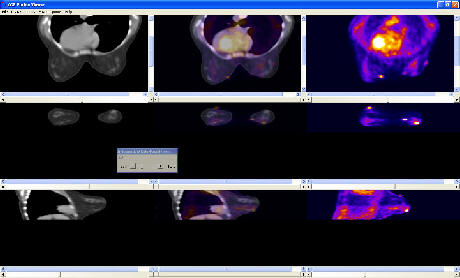
\includegraphics[width=1.00\textwidth]{multimodalbreastimage.png}
\caption{\label{fig:screenshot}A screenshot of a fused data set.
}
\end{figure}

To realise successful multimodal systems of the future, same key research challenges remain to be addressed. Among these challenges are the development of effective natural language processing, dialogue processing, and error-handling techniques. In addition, new multimodal systems will be needed for collaborative multiperson use. Before this new class of systems can proliferate, toolkits also will be needed to promote software development for both simulated and functioning systems.

Multimodal interfaces also are expected to be easier to learn and use, and they are preferred by users for many applications. They have the potential to expand computing to more challenging applications, to be used by a broader spectrum of clinicians, and accommodate more adverse usage conditions than in the past. This class of systems represents a relatively new direction for computing that draws from myriad input and output technologies currently becoming available.

\section{Overview}

Clinical user interfaces have been extensively discussed in the literature on information visualisation. MIMBCD-UI shows the details of an user interface for diagnosing breast cancer using multimodality medical imaging. MIMBCD-UI have several benefits. In fact, the diagnosis it self is more efficient since the clinical users may navigate using the overview of multimodality of imaging rather than the others techniques. The overview of multimodality of imaging window aids users in keeping track of their current position in the information space [8]. Moreover the overview window itself give users task-relevant information and a feeling of control [9]. A multimodality of views permits to acquire better, more efficient and flexible information and to easily diagnose in it; however, it is more difficult to users to manage information in a more complex user interface.

\section{Related Work}

This section describes existing work in the field of medical and clinical user interfaces.

\subsection{Patient Visualisation}

A two different interfaces to visualize patient histories on a PDA [2] describes two different users interfaces for mobile device tool that displays patient histories and permits to visually query patient data stored in hospital database.

\clearpage

% Commands to include a figure:
\begin{figure}[!hbt]
\centering
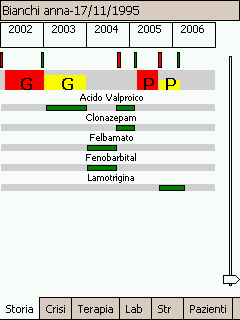
\includegraphics[width=0.50\textwidth]{zoomable.png}
\caption{\label{fig:zoomable}Zoomable interface of PHiP.
}
\end{figure}

The objective of this work is to display as much as possible information about the patient history on a limited display space, providing overview data as well as details. By displaying on a single screen of a personal computer the overview of multiple facets of records will provide users with a better sense of type and volume of available data.

In fact, PHiP (Patient History in Pocket) [2] is a tool designed for a mobile device that displays patient histories and permits to visually query patient data stored in the hospital database exploiting information visualisation techniques where it is able to accommodate on the screen a good amount of clinical cases.

This work has been developed according to an user-centered approach and will bring MIMBCD-UI support in that way. Beside the user studies conducted in the hospital at the requirement phase, they have performed with doctors evaluations of the different prototypes and this kind of information is kindly useful for our research field as well.

\clearpage

\subsection{Patient Progress}

In computer-assisted creation of patient progress notes [11] a prototype application that supports the creation of critical care notes by physicians in a hospital of an intensive care unit, called activeNotes, integrates automated, context-sensitive patient data retrieval and user control of automated data updates and alerts into the note creation process.

% Commands to include a figure:
\begin{figure}[!hbt]
\centering
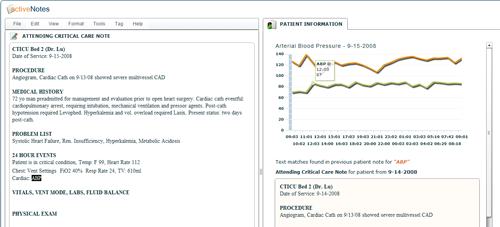
\includegraphics[width=1.00\textwidth]{activenotes.png}
\caption{\label{fig:activenotes}activeNotes Prototype System.
}
\end{figure}

A critical care note is a clinical document, written by a hospital physician, that documents and patient's progress and prognosis. This kind of work will help MIMBCD-UI project by giving us information analyse by physicians feedback and user understanding. It also bring us information with qualitative study by providing us the right path throw prototype design and user experience evaluation.

The physician-driven management of patient progress notes in an intensive care unit [20], describes a design exploration focused on techniques to support data input and management of electronic progress note content. This will help MIMBCD-UI project by giving us an alternative design exploration including observations, structured and semi-structured interviews, design and implementation of a prototype, and feedback gathered in qualitative study with physicians surveys.

\subsection{Interaction System}

On M/ORIS: a Medical/Operating Room Interaction System [12] is proposed an architecture for a real-time multimodal system, which provides non-contact, adaptive user interfacing for Computer-Assisted Surgery (CAS) [13]. This paper focuses on the proposed activity monitoring aspects of M/ORIS. The researchers have analyse the issues of Human-Computer Interaction (HCI) in an Operation Room (OR) based on real-world case studies.

% Commands to include a figure:
\begin{figure}[!hbt]
\centering
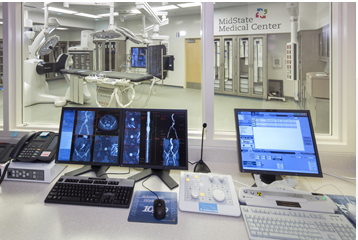
\includegraphics[width=1.00\textwidth]{moris.png}
\caption{\label{fig:moris}Operating room interaction system example.
}
\end{figure}

\clearpage

\subsubsection{CAS vs CAD}

Computer Aided Surgery (CAS) [14] and Computer Aided Diagnosis (CAD) [15] can contribute to the general cost cutting trend in health care by making it possible to have fewer staff perform the same activity in less time than with traditional methods. It also brings us human error prevention and, if so, the system can better audit the source of problems and reduce error effects. In particular, it is likely that in the near future, a single doctor will have to control and diagnose several computer-based processes during a surgical, diagnosis or clinical intervention.

Efficient User Interface (UI) design that matches the constrains of clinical environments and that helps reduce the doctor's workload will, in a large part, determine the success of CAS and CAD.

\subsubsection{User Interface for CAD}

CAD techniques, whether they enhance traditional methods (e.g. image visualisation [16]) or provide new tools such as augmented displays [10], share a common need for multimodality of imaging UI. Interface issues are systematically brought up in connection with new computer-assisted techniques, and poor UI design is cited [12, 16] as significant limiting factor for many operations. In particular, doctors criticise the lack of user-centered design, the difficulty to operate computer-assisted equipment during surgery, and the failure to convey information without otherwise constraining the doctor.

To address these issues, several authors have developed guidelines for medical UI design. An introduction to human factors in medical devices [17] and making medical device interfaces more user-friendly [18] stress the importance of a doctor-centered design for both efficiency and human error reduction. A framework for determining component and overall accuracy for computer assisted surgery systems [19] proposes a framework for evaluating the benefits of new UI paradigms in CAS system design that can be applied to CAD system design.

\clearpage

\subsection{Designing the User Interface}

Multimodal systems that process user's speech and pen-based gestural input have become a vital and expanding field, especially within the past years, with demonstrated advances in a growing number of research and application areas.

A growing interest in multimodal interface design is inspired in large part by the goals of supporting more transparent, flexible, efficient and powerfully expressive means of human-computer interaction that in the past. Multimodal interfaces are expected to support a wider range of diverse applications, be usable by a boarder spectrum of the average population, and function more reliably under realistic and challenging usage conditions.

In designing the user interface for multimodal speech and pen-based gesture applications: state-of-the-art systems and future research directions [21] article, researchers summarise the prevailing and emerging architectural approaches available for interpreting dual input signals in a robust manner, including early and late semantic fusion approaches, as well as new hybrid symbolic-statistical architecture, that potentially are capable of archiving very robust functioning, for processing pen-voice input (i.e. speech and gesture). Researchers also described a diverse collection od state-of-the-art multimodal systems that are capable of processing user's actions input. This will brings an enormous added value in the implementation and architecture of our future user interface.



\subsection{Usability and Ergonomic Testing}

Semiotic analysis combined with usability and ergonomic testing for evaluation of icons in medical user interface [3] have evaluated the medical icons and iconic interfaces of touch screen ventilator systems used in Intensive Care Unit (ICU).

The use of icons in iconic user interfaces [4] in medical devices like ventilator systems is a common practice. Precise communications through iconic interface between ventilator system and medical users like physicians or nurses is critical to avoid medical errors which may cost patient's life.

This research will help us understand and defining a set of icons that will represent our metaphor analysis throw this work. It also, but not less, give us the right information about usability testing where icons can be tested using various usability testing methods. At last it will help us getting information about Semiotic and Lexical Analysis.

Semiotics is a study of cultural sign processes, analogy, signification, communication, metaphors, signs and symbols [5]. A semiotic analysis is concerned with meaning, which stems from relationships - in particular, the among signs relationships [6].

Linguistics has a term - 'Lexical Analysis' which is the process of converting a sequence of characters into a sequence of tokens. A lexical analysis helped in classification of medical icons [7] into mainly three classes: icons, indices and symbols.

\section{Conclusions}

So far, there have been hardly any specific studies wherein the medical interfaces are tested and evaluated for their comprehensibility and usability to users. Pretty interfaces that hide the ugly reality of underlying data do not engender clinician trust and respect. New visual cues that provide immediate user insight into assumptions and deficiencies regarding the displayed information are required. Clinicians expect and interface to keep clear and direct with easy and intuitive usability.

Finally, some requirements for advancing innovative imaging multimodality are not just intellectual ones, but rather social, political, and educational in nature. The development of state-of-the-art of multimodal images user interface of this kind also requires multidisciplinary expertise in a variety of areas, such as human factors and ergonomics [22], perception and graphics, linguistics, psychology, pattern recognition, statistics, engineering and computer science. The multidisciplinary nature of this research across the entire spectrum.

\clearpage

\begin{thebibliography}{}

% 1
\bibitem{} Michael G. Kahn, Janette Coble, and Matthew Orland. 1998. Keep no secrets and tell no lies: computer interfaces in clinical care. In \emph{CHI 98 Cconference Summary on Human Factors in Computing Systems} (CHI '98). ACM, New York, NY, USA, 100-101. DOI=http://dx.doi.org/10.1145/286498.286553

% 2
\bibitem{} Carmelo Ardito, Paolo Buono, Maria Francesca Costabile, and Rosa Lanzilotti. 2006. Two different interfaces to visualize patient histories on a PDA. In \emph{Proceedings of the 8th conference on Human-computer interaction with mobile devices and services} (MobileHCI '06). ACM, New York, NY, USA, 37-40. DOI=http://dx.doi.org/10.1145/1152215.1152223

% 3
\bibitem{} Ganesh Bhutkar, Ravi Poovaiah, Dinesh Katre, and Shekhar Karmarkar. 2011. Semiotic analysis combined with usability and ergonomic testing for evaluation of icons in medical user interface. In \emph{Proceedings of the 3rd International Conference on Human Computer Interaction} (IndiaHCI '11). ACM, New York, NY, USA, 57-67. DOI=http://dx.doi.org/10.1145/2407796.2407804

% 4
\bibitem{} Katre Dinesh. 2004. Experimenting with Uniface: A Tool for
Usability Testing of Icons. \emph{National Usability Conference} (ACM-SIGCHI-SI). Easy 2004, Bangalore, India.

% 5
\bibitem{} \emph{http://en.wikipedia.org/wiki/Semiotics\#Terminology} retrieved
on 2nd Nov. 2010.

% 6
\bibitem{} \emph{http://www.uk.sagepub.com/upmdata/5171\_Berger\_Final\_Pages\_Chapter\_1.pdf} retrieved on 18th Oct. 2010.

% 7
\bibitem{} Poovaiah Ravi. 1995. Graphic Symbols for Environmental
Signage: A Design Perspective. \emph{International Symposium on
Public Graphics}, The Netherlands.

% 8
\bibitem{} Plaisant, C., Carr, D., and Shneiderman, B. Image browsers:
Taxonomy, guidelines, and informal specifications. \emph{IEEE
Software, 12(2)}, 1995, 21-32.

% 9
\bibitem{} Shneiderman, B. Designing the User Interface. \emph{AddisonWesley},
Reading, MA:1998.

% 10
\bibitem{} Daniel Cukier and Joseph W. Yoder. 2011. The artist in the computer scientist: more humanity to our research. In \emph{Proceedings of the 10th SIGPLAN symposium on New ideas, new paradigms, and reflections on programming and software} (Onward! 2011). ACM, New York, NY, USA, 129-136. DOI=http://dx.doi.org/10.1145/2089131.2089134

% 11
\bibitem{} Lauren Wilcox, Jie Lu, Jennifer Lai, Steven Feiner, and Desmond Jordan. 2009. ActiveNotes: computer-assisted creation of patient progress notes. In \emph{CHI '09 Extended Abstracts on Human Factors in Computing Systems} (CHI EA '09). ACM, New York, NY, USA, 3323-3328. DOI=http://dx.doi.org/10.1145/1520340.1520480

% 12
\bibitem{} Sébastien Grange, Terrence Fong, and Charles Baur. 2004. M/ORIS: a medical/operating room interaction system. In \emph{Proceedings of the 6th international conference on Multimodal interfaces} (ICMI '04). ACM, New York, NY, USA, 159-166. DOI=http://dx.doi.org/10.1145/1027933.1027962

% 13
\bibitem{} Horst K. Hahn, Bernhard Preim, Dirk Selle, and Heinz Otto Peitgen. 2001. Visualization and interaction techniques for the exploration of vascular structures. In \emph{Proceedings of the conference on Visualization '01} (VIS '01). IEEE Computer Society, Washington, DC, USA, 395-402.

% 14
\bibitem{} Computer\-assisted surgery: \emph{https://en.wikipedia.org/wiki/Computer\-assisted\_surgery} retrieved on 08th May. 2016.

% 15
\bibitem{} Computer-aided diagnosis: \emph{https://en.wikipedia.org/wiki/Computer\-aided\_diagnosis} retrieved on 08th May. 2016.

% 16
\bibitem{} F. Vogt, S. Krüger, H. Niemann and C. Schick, "A System
for Real-Time Endoscopic Image Enhancement", R.E. Ellis
and T.M. Peters (Eds.), \emph{MICCAI 2003}, LNCS 2879, pp. 356–
363, 2003.

% 17
\bibitem{} D. Sawyer, K. J. Aziz, C. L. Backinger, E. T. Beers, A.
Lowery and S. M. Sykes, “An Introduction to Human
Factors in Medical Devices”, \emph{US Department of Health and
Human Services, Public Health Service, Food and Drug
Administration, Center for Devices and Radiological Health}; 1996.

% 18
\bibitem{} M. E. Wicklund, “Making Medical Device Interfaces More
User-Friendly”, \emph{Medical Device and Diagnostic Industry}; 1998.

% 19
\bibitem{} A. B. Mor, J. E. Moody, D. Davidson, R. S. Labarca, B.
Jaramaz, and A. M. Digioia III, "A Framework for
Determining Component and Overall Accuracy for
Computer Assisted Surgery Systems", R.E. Ellis and T.M.
Peters (Eds.), \emph{MICCAI 2003}, LNCS 2879, pp. 985−986,
2003.

% 20
\bibitem{} Lauren Wilcox, Jie Lu, Jennifer Lai, Steven Feiner, and Desmond Jordan. 2010. Physician-driven management of patient progress notes in an intensive care unit. In \emph{Proceedings of the SIGCHI Conference on Human Factors in Computing Systems} (CHI '10). ACM, New York, NY, USA, 1879-1888. DOI=http://dx.doi.org/10.1145/1753326.1753609

% 21
\bibitem{} Sharon Oviatt, Phil Cohen, Lizhong Wu, John Vergo, Lisbeth Duncan, Bernhard Suhm, Josh Bers, Thomas Holzman, Terry Winograd, James Landay, Jim Larson, and David Ferro. 2000. Designing the user interface for multimodal speech and pen-based gesture applications: state\-of\-the\-art systems and future research directions. \emph{Hum.\-Comput. Interact. 15, 4} (December 2000), 263\-322. DOI=http://dx.doi.org/10.1207/S15327051HCI1504\_1

% 22
\bibitem{} \emph{https://en.wikipedia.org/wiki/Human\_factors\_and\_ergonomics} retrieved on 08th May. 2016.

% 23
\bibitem{} Jose Luis Pelaez, Inc./CORBIS. Ethics Manual – Principal Features of Medical Ethics: Physicians and Patients (chapter two) at. \emph{http://www.wma.net/en/30publications/30ethicsmanual/pdf/chap\_2\_en.pdf}.

\end{thebibliography}
\end{document}